\section{Resoconto attività di verifica}
\subsection{Revisione dei requisiti}
\subsubsection{Analisi statica dei documenti}
Tutta la documentazione prodotta in ingresso alla Revisione dei Requisiti è stata sottoposta ad una meticolosa attività di verifica
basata su quanto previsto all'interno del documento delle norme di progetto
Questa attività è stata espletata dai verificatori.

\subsubsection{Analisi automatizzata dei documenti}
Al fine di verificare la qualità della documentazione prodotta il gruppo ha deciso di addotare come metrica di verifica
l'indice di Gulpease generato grazie ad un processo automatizzato configurato in GitHub, unitamente alla generazione di un indice di 
correttezza grammaticale del testo.
Di seguito sono presentati i due grafici rappresentativi dei valori ottenuti dall'analisi dei documenti sino all'approvazione degli stessi.
Per quanto riguarda i verbali redatti in occasione dei meeting tra i membri del gruppo e con i proponenti si espongono i valori in forma tabellare


\begin{center}
   
		\begin{figure}[!htb]
			\centering
			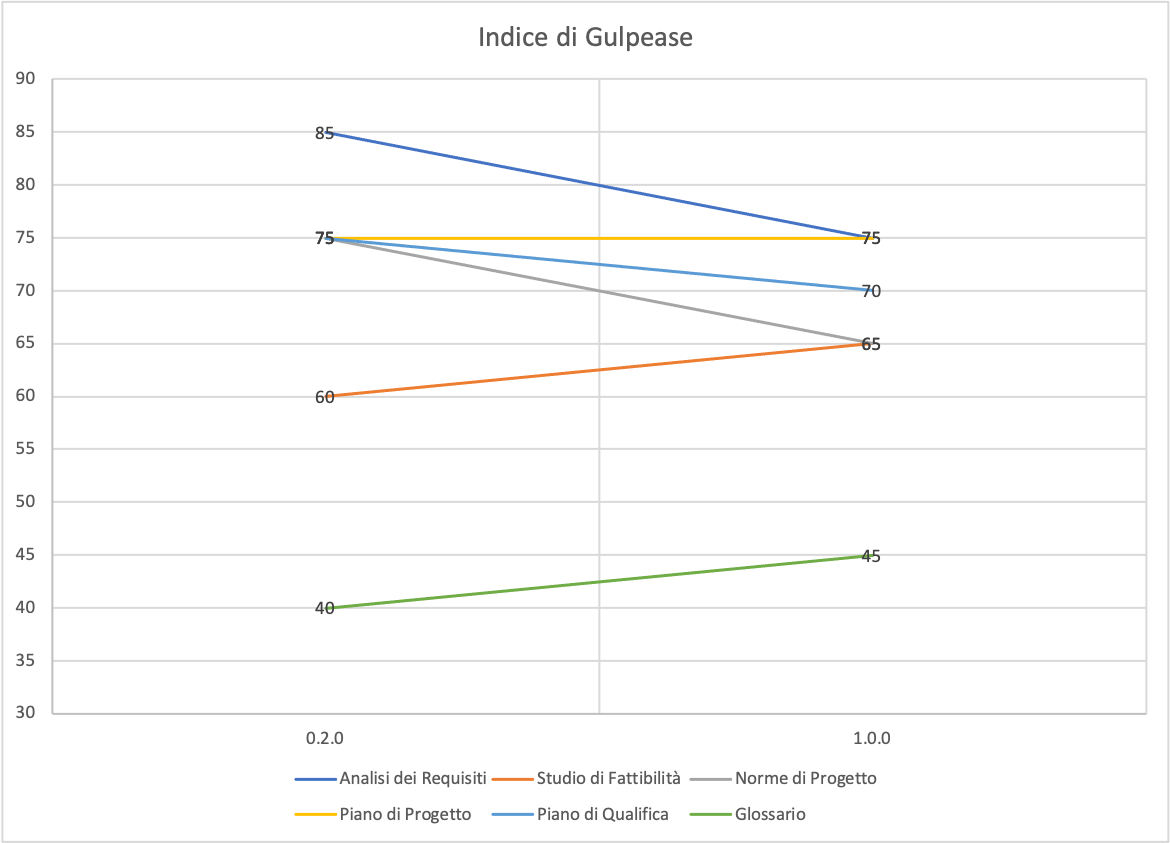
\includegraphics[scale=0.80]{res/images/grafico_gulpease.png}	
			\caption{Grafico Indice di Gulpease}
        \end{figure}
        

        \begin{figure}[!htb]
			\centering
			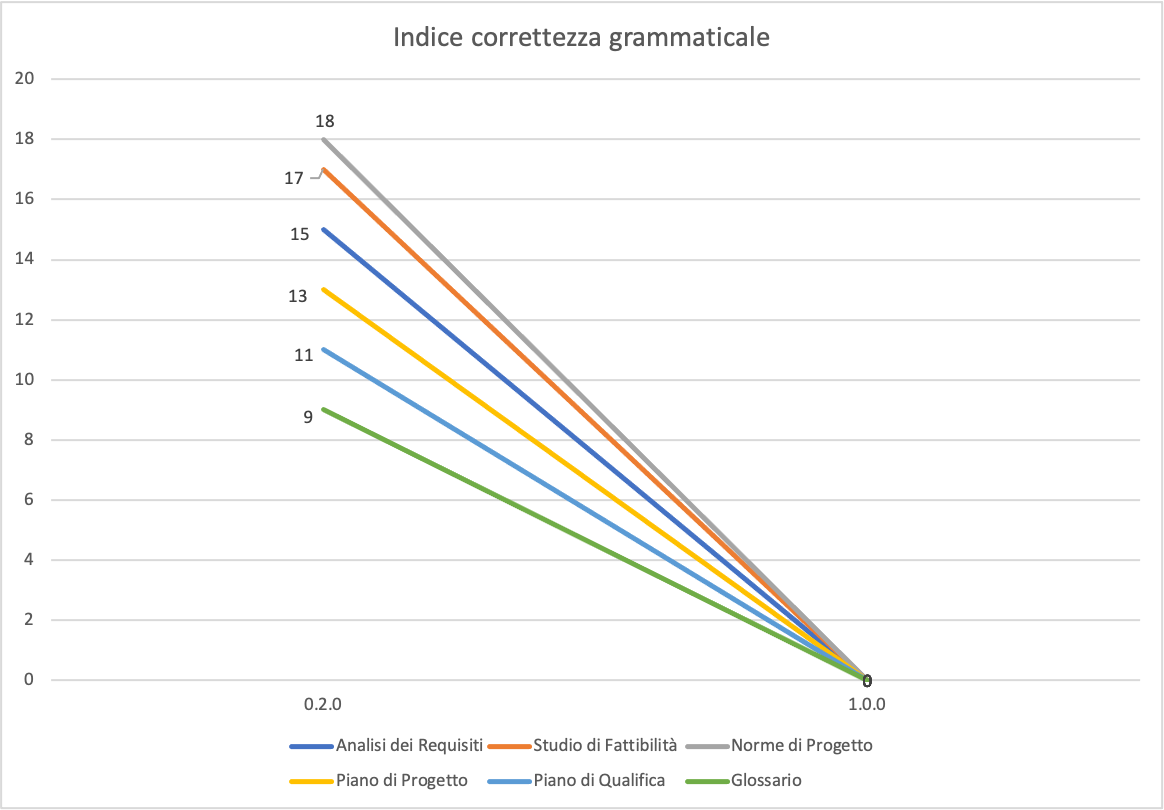
\includegraphics[scale=0.80]{res/images/grafico_correttezza.png}	
			\caption{Grafico indice correttezza grammaticale}
		\end{figure}
	




    \begin{center}
        \rowcolors{1}{white}{blue!20}
        
        \begin{longtable}{|c|c}
      
        \hline
        \rowcolor{lighter-grayer}
        \textbf{Documento} & \textbf{Indice di Gulpease} \\
       
        \hline
        \endfirsthead


        \hline

        Verbale Interno 2020-12-02 & 60 \\
        Verbale Intero 2020-12-07& 61  \\
        Verbale Estero 2020-12-10 & 63  \\
        Verbale Interno 2020-12-14 & 62 \\
        Verbale Interno 2020-12-17 & 62  \\
        Verbale Interno 2020-12-22 & 60 \\
        Verbale Interno 2021 & 0  \\
        Verbale Interno 2021 & 0\\  

    
        \hline

        \caption{Indice di Gulpease dei verbali}
        
        \end{longtable}
    \end{center}
\end{center}


